% Thermodynamic PV Diagrams
% Demonstrates: Carnot cycle, isotherms, adiabats, and work shading on PV plot.
% Compile with: pdflatex main.tex

\documentclass[border=10pt]{standalone}
\usepackage{tikz}
\usepackage{pgfplots}
\pgfplotsset{compat=1.18}
\usetikzlibrary{arrows.meta, patterns, calc, decorations.markings}
\usepackage{amsmath}

\begin{document}
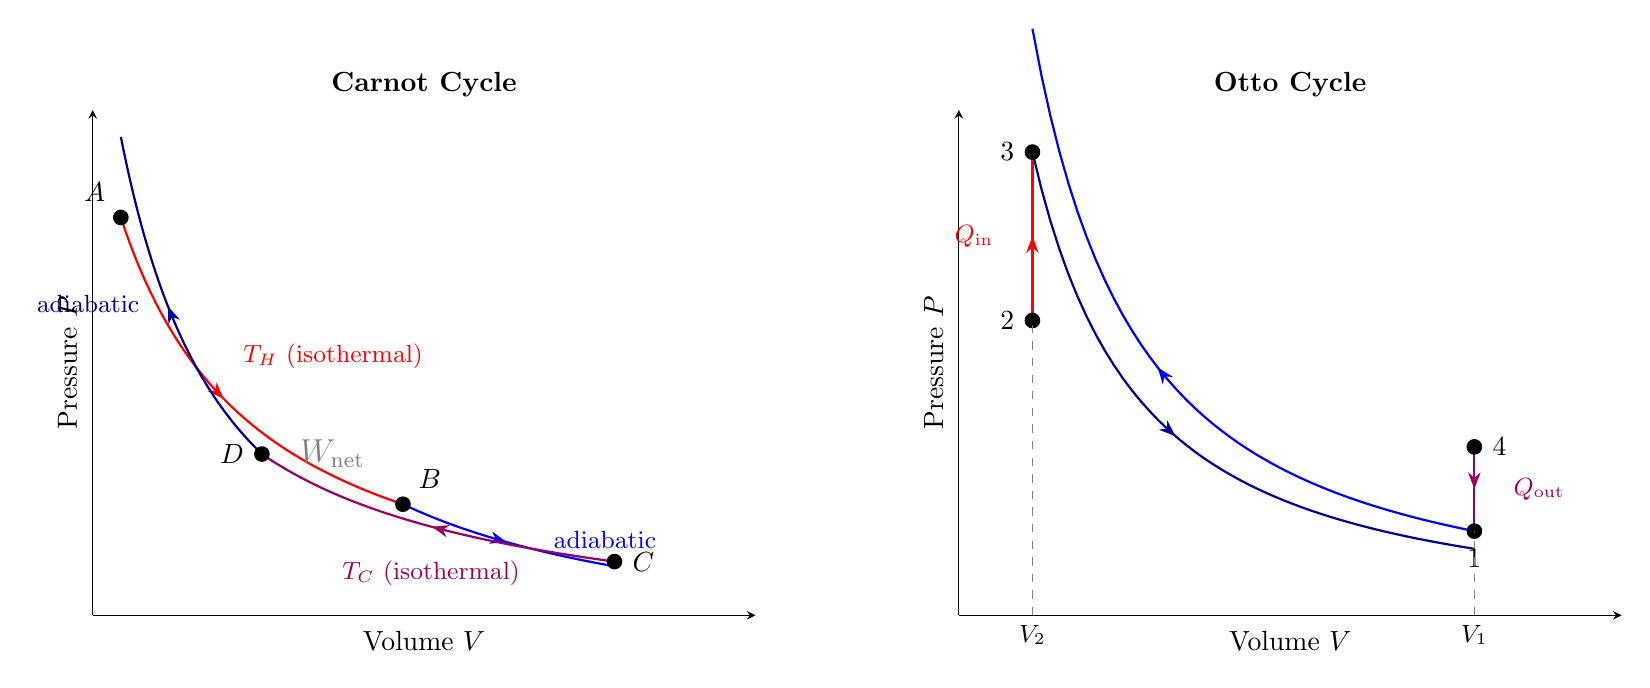
\begin{tikzpicture}

% =============================================================================
% Diagram 1: Carnot Cycle
% =============================================================================
\begin{scope}[shift={(0,0)}]
\begin{axis}[
    width=10cm, height=8cm,
    title={\textbf{Carnot Cycle}},
    xlabel={Volume $V$},
    ylabel={Pressure $P$},
    xmin=0.8, xmax=5.5,
    ymin=0.3, ymax=5,
    xtick=\empty, ytick=\empty,
    axis lines=left,
    clip=false,
    every axis title/.style={at={(0.5,1.05)}},
]

    % State points (approximate ideal gas behavior)
    % A(1,4), B(3,2), C(4.5,0.8), D(2,1.5)

    % --- Isothermal expansion A→B (hot, T_H) ---
    \addplot[thick, red, domain=1:3, samples=50,
        postaction={decorate, decoration={
            markings, mark=at position 0.5 with {\arrow{Stealth[length=6pt]}}
        }}]
        {4/x};
    \node[red, above right, font=\small] at (axis cs:1.8,2.5) {$T_H$ (isothermal)};

    % --- Adiabatic expansion B→C ---
    \addplot[thick, blue, domain=3:4.5, samples=50,
        postaction={decorate, decoration={
            markings, mark=at position 0.5 with {\arrow{Stealth[length=6pt]}}
        }}]
        {4*3^0.4/(x^1.4)};
    \node[blue, right, font=\small] at (axis cs:4,1) {adiabatic};

    % --- Isothermal compression C→D (cold, T_C) ---
    \addplot[thick, red!60!blue, domain=4.5:2, samples=50,
        postaction={decorate, decoration={
            markings, mark=at position 0.5 with {\arrow{Stealth[length=6pt]}}
        }}]
        {3.6/x};
    \node[red!60!blue, below, font=\small] at (axis cs:3.2,0.9) {$T_C$ (isothermal)};

    % --- Adiabatic compression D→A ---
    \addplot[thick, blue!60!black, domain=2:1, samples=50,
        postaction={decorate, decoration={
            markings, mark=at position 0.5 with {\arrow{Stealth[length=6pt]}}
        }}]
        {3.6*2^0.4/(x^1.4)};
    \node[blue!60!black, left, font=\small] at (axis cs:1.2,3.2) {adiabatic};

    % --- State labels ---
    \node[circle, fill=black, inner sep=2pt, label=above left:{$A$}]
        at (axis cs:1,4) {};
    \node[circle, fill=black, inner sep=2pt, label=above right:{$B$}]
        at (axis cs:3,{4/3}) {};
    \node[circle, fill=black, inner sep=2pt, label=right:{$C$}]
        at (axis cs:4.5,{3.6/4.5}) {};
    \node[circle, fill=black, inner sep=2pt, label=left:{$D$}]
        at (axis cs:2,{3.6/2}) {};

    % --- Work annotation ---
    \node[font=\large, text=gray] at (axis cs:2.5,1.8) {$W_{\text{net}}$};

\end{axis}
\end{scope}

% =============================================================================
% Diagram 2: Otto Cycle (gasoline engine)
% =============================================================================
\begin{scope}[shift={(11,0)}]
\begin{axis}[
    width=10cm, height=8cm,
    title={\textbf{Otto Cycle}},
    xlabel={Volume $V$},
    ylabel={Pressure $P$},
    xmin=0.5, xmax=5,
    ymin=0, ymax=6,
    xtick=\empty, ytick=\empty,
    axis lines=left,
    clip=false,
    every axis title/.style={at={(0.5,1.05)}},
]

    % State points: 1(4,1), 2(1,3.5), 3(1,5.5), 4(4,2)

    % --- Adiabatic compression 1→2 ---
    \addplot[thick, blue, domain=4:1, samples=50,
        postaction={decorate, decoration={
            markings, mark=at position 0.5 with {\arrow{Stealth[length=6pt]}}
        }}]
        {1*4^1.4/(x^1.4)};

    % --- Constant-volume heat addition 2→3 ---
    \draw[thick, red, postaction={decorate, decoration={
        markings, mark=at position 0.5 with {\arrow{Stealth[length=6pt]}}
    }}] (axis cs:1, 3.5) -- (axis cs:1, 5.5);
    \node[red, left, font=\small] at (axis cs:0.8, 4.5) {$Q_{\text{in}}$};

    % --- Adiabatic expansion 3→4 ---
    \addplot[thick, blue!60!black, domain=1:4, samples=50,
        postaction={decorate, decoration={
            markings, mark=at position 0.5 with {\arrow{Stealth[length=6pt]}}
        }}]
        {5.5*1^1.4/(x^1.4)};

    % --- Constant-volume heat rejection 4→1 ---
    \draw[thick, red!60!blue, postaction={decorate, decoration={
        markings, mark=at position 0.5 with {\arrow{Stealth[length=6pt]}}
    }}] (axis cs:4, 2) -- (axis cs:4, 1);
    \node[red!60!blue, right, font=\small] at (axis cs:4.2, 1.5) {$Q_{\text{out}}$};

    % --- State labels ---
    \node[circle, fill=black, inner sep=2pt, label=below:{$1$}]
        at (axis cs:4,1) {};
    \node[circle, fill=black, inner sep=2pt, label=left:{$2$}]
        at (axis cs:1,3.5) {};
    \node[circle, fill=black, inner sep=2pt, label=left:{$3$}]
        at (axis cs:1,5.5) {};
    \node[circle, fill=black, inner sep=2pt, label=right:{$4$}]
        at (axis cs:4,2) {};

    % --- Volume labels ---
    \draw[dashed, gray] (axis cs:1,0) -- (axis cs:1,3.5);
    \draw[dashed, gray] (axis cs:4,0) -- (axis cs:4,1);
    \node[below, font=\small] at (axis cs:1,0) {$V_2$};
    \node[below, font=\small] at (axis cs:4,0) {$V_1$};

\end{axis}
\end{scope}

\end{tikzpicture}
\end{document}
